\documentclass[11pt]{article}
\usepackage{a4wide}
\usepackage{float}
\usepackage{graphicx}
\usepackage{hyperref}
\usepackage[margin=1in,footskip=0.25in]{geometry}
\graphicspath{{./images/}}

\begin{document}

\begin{titlepage}
\title{Reinforcement learning gebaseerde agent voor presidenten}
\author{Freya Van Speybroek \& Thor Dossche}
\date{Academiejaar 2020 \- 2021}
\maketitle
\thispagestyle{empty}
\end{titlepage}


\section{Inleiding}
In dit project zullen we bestuderen hoe reinforcement learning kan toegepast worden op een kaartspel. Het kaartspel dat we gaan bekijken is presidenten. Dit is een perfect voorbeeld van een spel waarbij we incomplete informatie hebben: er kan namelijk niet in de kaarten van de tegenstanders gekeken worden. Daarbij is elke toestand discreet, waardoor het probleem kan gemodelleerd worden als een Partially Observable Markov Decision Process (POMDP).\\\\
Voor dit soort problemen zijn er al heel wat oplossingsmethodes, waarvan we er een paar zullen uitproberen en vergelijken. Daarbij kunnen we ons ook de vraag stellen of het wel degelijk rendeert om Reinforcement Learning te gebruiken, misschien zijn we beter af met een heuristiek? 

\subsection{Het probleem}
Presidenten kent veel varianten, de regels liggen namelijk niet hard vast en kunnen daarom vaak besproken worden onder de spelers. Afhankelijk van welke regels je gebruikt, kan het spel moeilijker worden. \\\\
Bij het spelen van presidenten speel je meerdere spelletjes. Na ieder spel zullen de `rangen' voor het volgend spel gekend zijn. Ieder spel bestaat uit meerdere rondes. In deze rondes proberen de spelers zoveel mogelijk kaarten te leggen om zo al hun kaarten uit te spelen. Tijdens een ronde moeten spelers elk om beurt een kaart leggen hoger of gelijk aan de vorige kaart. Het aantal van die kaarten moet hoger of gelijk zijn aan de kaart(en) van de vorige beurt.\\
Als een speler geen kaart(en) meer kan of wil liggen past hij, eenmaal gepast zal hij niet meer aan de beurt komen in de ronde. Als alle spelers op een na gepast hebben is de winnaar van de ronde gekend. Deze speler mag een nieuwe ronde starten met een kaart of kaarten naar keuze. Als een speler al zijn kaarten heeft uitgespeeld krijgt hij een rang toegewezen voor het volgende spel.\\
De persoon die het eerste uitspeelt is de president, de tweede de vice-president.
De persoon die als laatste overblijft is de scum, degene die als voorlaatste uitspeelt is de vice-scum.\\
Als alle rangen gekend zijn start het volgende spel. Na het delen van de kaarten krijgt de president de beste 2 kaarten van de scum, de scum krijgt de 2 slechtste van de president. Hetzelfde geldt voor vice-president en vice-scum, maar die wisselen slechts 1 kaart uit.\\\\
Nog enkele basisregels:\\\\
- De speler die de ‘klaver 3’ heeft, start de eerste ronde van een spel met deze kaart (of meerdere kaarten van waarde 3 waaronder de `klaver 3'). \\
- Als een speler uit is, dan wordt een nieuwe ronde gestart en mag de speler links van de net uitgespeelde speler beginnen.\\\\
Om het spel interessanter te maken hebben wij nog een paar extra regels toegevoegd:\\\\
- Als een 7 is gespeeld, dan moet de volgende kaart lager of gelijk zijn aan die 7 ook het aantal kaarten moet gelijk zijn aan het aantal gelegde kaarten.\\
- De kaart 2 is een joker die kan gebruikt worden als hoogste kaart in het spel, of als een extra kaart. Als de joker gelegd wordt samen met een kaart van een andere waarde zal de joker deze waarde aannemen.\\
- De ranking van de kaarten is dus als volgt: 3,4,5,6,7,8,9,10,V,Q,K,A,2\\

\subsection{De environment}
Bij Reinforcement Learning gaan we niet aan de slag met een dataset, maar met een “environment”, die het spel zelf voorstelt. We willen dan een agent bekomen die een zo hoog mogelijke score behaalt in de environment. \\
In dit geval, willen we een agent die zo vaak mogelijk of zo lang mogelijk president kan zijn. Maar, de situatie is niet zo zwart-wit. Het is namelijk ook goed zijn om veel vice-president te zijn want dan ben je nog steeds in een voordeelpositie. Goed spelen kan ook zijn dat je met zeer slechte kaarten toch niet scum wordt maar door tactisch te spelen de high-scum rang behaalt. Soms krijg je gewoon kaarten waarmee je gewoon niet kan winnen hoe goed je ook bent, heb je dan slecht gespeeld als je scum wordt? Het is duidelijk niet zo dat dat altijd winnen een goeie maat is om te meten of je goed bent. Er zal dus gezocht moeten worden naar een goed evenwicht van deze verschillende factoren om te bepalen of de agent goed is. \\
Bovendien kan de environment ook op veel verschillende manieren bekeken worden. Hoe wordt een state voorgesteld, welke rewards delen we uit, welke acties maken we mogelijk? Dit zijn allemaal deelproblemen op zich, waarvoor we verschillende oplossingen zullen proberen vinden.\\\\

\subsection{Mogelijke oplossingsmethoden}
Zoals in de inleiding besproken, is ons probleem gemodelleerd als  een Partially Observable Markov Decision Process (POMDP). Hier zijn verschillende oplossingsmethoden voor mogelijk, waaronder Q-learning, DQN en Monte Carlo Tree Search. Het doel van deze oplossingsmethoden en van Reinforcement Learning zelf, is om een agent, gegeven een toestand en een aantal acties, de meest optimale actie te laten kiezen. Hierbij wordt met optimaal bedoeld dat de agent zijn score maximaliseert. Een actie uitvoeren in een bepaalde state, geeft de agent dus een reward (die goed of slecht kan zijn).\\\\ 
Een eerste interessante weg is Q-learning. Alhoewel dit een algoritme is dat we vaak bij simpele spelsituaties gebruikt zien (zoals \cite{simple-qlearning}), zouden we kunnen kijken of dit goede resultaten geeft. Aangezien Q-learning werkt met een Q-table die per state en per actie een score bijhoudt, kan het toch zijn dat dit te beperkt is voor de grote aantal mogelijke spelsituaties in presidenten. \\\\
Het is daarom misschien interessanter om met een DQN of Deep Q-Network te werken, waarmee we kunnen werken met grotere states om zo meer informatie over het spel bij te houden. Een succesvol voorbeeld met neurale netwerken is \cite{nn-paper}, waar ze werken met spel dat een gelijkaardige complexiteit heeft als presidenten. Waarom ze niet met DQN werken, wordt ook besproken, en is interessant om later in dit onderzoek nog eens aan te halen. \\\\
Ten laatste zou Monte Carlo Tree Search een zelfde beperkingen geven als Q-learning, namelijk de grootte van de state. Hoe groot kunnen we de state maken tot we in een situatie komen waar we te veel paden hebben om te simuleren? Hiervoor zijn er wel al oplossingen, waaronder Partially Observable Monte-Carlo Planning (POMCP), wat een aangepaste Monte Carlo tree search is om POMDPs op te lossen \cite{mct-1}. Er bestaan ook andere manieren door Monte Carlo te combineren met andere oplossingen, zoals in \cite{mct-2} of \cite{mct-3}.\\\\

\section{Methodiek}
Uit de bovenstaande besproken oplossingsmethodes, bespreken we de eerste twee, namelijk Q-learning en DQN. Interessant hieraan is dat de tweede methode, die met een Deep Q-Network werkt, gebaseerd is op het Q-learning van de eerste methode. Ook bekijken we een alternatieve, eenvoudigere oplossingsmethode die aan de hand van heuristieken of vuistregels van presidenten werkt.\\

\subsection{Heuristiek}

Om te toetsen hoe goed de andere oplossingsmethoden zijn, hebben we een goede speler nodig. Hiervoor hebben we een heuristiek geimplementeerd die ongeveer volgt wat echte spelers in het spel zouden doen, namelijk:\\
\begin{itemize}
	\item Leg altijd de laagste kaart mogelijk. Als je meerdere van die kaart hebt, leg ze allemaal.
	\item Leg enkel een joker als je niet anders kan.
	\item Pas enkel wanneer je niets kan leggen.
\end{itemize}
Een echte speler zal natuurlijk ook rekening houden met details zoals welke kaarten al gelegd zijn doorheen het spel, hoeveel spelers al uitgespeeld zijn, ... Maar we zullen toch zien dat deze heuristiek opvallend goede resultaten behaald. \\\\
Ook hebben we een extra speler geimplementeerd: de random speler. Deze speler kiest een willekeurige zet uit de mogelijke zetten die hij op dat moment kan doen gegeven de laatst gelegde kaart(en) en de kaarten in zijn hand. Zo hebben we nu een goede en slechtere speler, waarop getest kan worden.\\\\

\subsection{Q-learning}
\subsubsection{Theorie}
Q-learning helpt ons zoeken naar een zo goed mogelijke policy \textbf{(todo: leg policy uit? zie dqn-pract)}. De letter $Q$ slaat op de functie die gebruikt wordt om, gegeven een state en een actie, de waarde van deze combinatie te vinden. Deze waarde geeft aan hoe goed - of slecht - een bepaalde actie is in een bepaalde state.\\\\
Op basis van de Bellman equations \cite{bellman-equations}, kunnen we een update regel definieren die er als onderstaande formule uitziet. Een Q-waarde van een bepaald state-actie paar zal dus veranderen met de tijd. Daarom moeten we in het begin de Q-waarden initialiseren, om die dan wanneer nodig aan te passen.\\\\


\begin{figure}[h]
\centering
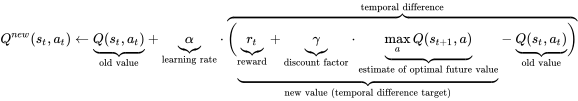
\includegraphics[scale=0.70]{images/qformula.png}
\caption{Q function - Source: wikipedia.org/wiki/Q-learning}
\label{fig:qfunction}
\end{figure}

Er zijn nog een aantal belangrijke parameters aanwezig in de formule. 
\begin{itemize}
	\item Learning rate: Geeft aan in welke mate we de Q-waarde updaten, een grote learning rate zal dus meer impact hebben op de uiteindelijke Q-waarde dan een kleinere.
	\item Reward: Score die berekend wordt op basis van de state waar we in waren en de gekozen actie. Door deze actie uit te voeren, komen we in een nieuwe state en kunnen we kijken hoe waardevol deze actie was. 
	\item Discount factor: Geeft aan hoe belangrijk toekomstige rewards zijn. Een hoge discount factor zal meer belang hechten aan rewards over een lange tijd, een lage discount factor laat het algoritme enkel rewards in een korte tijdsperiode beschouwen.
	\item Estimate of optimal future value: In deze stap gaan we de Q-waarden overlopen over alle mogelijke acties in de volgende state, en halen we de hoogste Q-waarde eruit. Merk op dat als de discount factor 0 is, dit niet uitmaakt, en dus niet naar toekomstige states of rewards kijken.
\end{itemize}

Daarbij is het in Q-learning belangrijk om te beschouwen hoe we de volgende actie a kiezen, om dan overeenkomende $Q(s,a)$ aan te passen. We zouden elke keer de beste actie kunnen kiezen op basis van de Q-waardem, maar dit zal in begin niet werken, aangezien er dan nog helemaal niets geleerd is. We willen dus genoeg exploratie hebben, zeker in het begin! Een oplossing hiervoor is om een $\epsilon$-greedy policy te volgen. Waarbij we met kans $\epsilon$ een willekeurige actie kiezen, en met kans $1-\epsilon$ een actie kiezen gebaseerd op de huidige policy. We kunnen deze $\epsilon$ eventueel laten variëren met de tijd.\\

\subsubsection{Implementatie}
De Q-waarden die doorheen het algoritme geupdate worden, worden bijgehouden in een Q-table. In onze eerste implementatie houdt de state 2 velden bij die de laatst gelegde kaart en zijn hoeveelheid voorstellen. De state wordt gegeven als een tuple (rang, aantal), en acties worden op dezelfde manier voorgesteld. Zo indexeren we de Q-table met deze 2 tuples. \\\\
We kunnen natuurlijk bediscussiëren of het niet beter zou zijn om een grotere state bij te houden, maar hier komen we later bij onze testresultaten op terug. Er is wel een beperking in hoe groot we de state kunnen maken, aangezien er een punt zou zijn waar de tabel zo groot wordt dat veel states niet meer bezocht worden. \\\\
De initiele Q-waarden in de tabel zijn 0 voor alle acties behalve `skip'. Vanaf nu zullen we het over een skip hebben als het over een beurt passen gaat. De waarden voor skip in elke mogelijke state wordt op -1 gezet, wat betekent dat we die al in het begin afstraffen. Op deze manier proberen we ervoor te zorgen dat de agent zo veel mogelijk beslist om wel een kaart te leggen. \\\\
Aangezien we hier de state beperkt moeten houden, moeten we best ook de taktiek van de agent beperkt houden, door hem op zo een goed mogelijke manier de rondes te laten spelen spelen, en niet te kijken naar winnen van het spel. Natuurlijk zal je het spel vaak winnen als je goed speelt in rondes. Dit is ook wat onze heuristieke speler doet. Welke reward functie we daaroor implementeren zullen we bespreken bij resultaten.\\\\
Ook hebben we een poging gedaan om de state-acties in een bitvector vorm te beschrijven. Dit omdat als we met grotere states en acties werken we zo meer geheugen zouden besparen dan gebruik te maken van tuples. Echter bleek dat dit negatief was, ook voor meer uitgebreide state-actie representaties, voor de performantie van het trainen en geen significante verbeteringen bijbracht in de prestatie van de agent. Daarom zijn we van dit idee afgestapt.\\


\subsection{Deep Q-Network}
\subsubsection{Theorie}
In plaats van de tabel letterlijk op te slaan en up te daten, benaderen we in het DQN-algoritme de tabel met een functie-approximator. Deze functie-approximator is een neuraal netwerk.\\\\
Het updaten van dit neuraal netwerk werkt dan als volgt. Stel we bevinden ons in een toestand $s$, dan wordt er een actie $a$ gekozen op basis van een $\epsilon$-greedy policy. Door deze actie uit te voeren, komen we in een nieuwe state $s'$ terecht en krijgen we ook een reward $r$. Waar we bij Q-learning hiermee de Q-table kunnen updaten, is het hier niet zo simpel. \\\\
De volgende stap is om deze originele state, de actie, de nieuwe state en de reward op te slaan in een replay memory. In dit replay memory krijgen we dus een verzameling van tuples van de vorm $(s,a,r,s')$. In elke stap nemen we dan samples uit het replay memory en stellen we targets op. Deze targets worden ongeveer dezelfde manier berekend als de temporal difference targets bij Q-learning (zie Figure ~\ref{fig:qfunction}). Enkel is hier het verschil dus dat $Q$ nu een functie-approximator is. Daarbij zien we dat deze targets van de vorm `reward + estimate of optimal future value' zijn. Dit tweede deel is niet meer nodig als we aan het einde van de episode zijn, dan houden we dus enkel de reward over als target. \\\\
Daarna wordt het netwerk geupdate met de MSE-loss functie, en kunnen we dit allemaal herhalen.\\\\

\subsubsection{Implementatie}
Gelukkig moeten we hier niet het warm water opnieuw uitvinden, en zijn er al een aantal frameworks ter beschikking die ons een handje kunnen helpen. Wij hebben gekozen voor PyTorch, die dus de implementatie details voor zich neemt.\\\\
Het belangrijkste was hier om te beslissen hoe we precies ons netwerk gingen voorstellen: welke inputs, hidden layers en outputs hebben we nodig?\\\\
Ons initieel idee was om niet te beginnen met een te grote state, om te kijken of we toch resultaten gelijkaardig aan de heuristieke speler konden krijgen met dezelfde informatie. Daarom hebben we gekozen om de de kaarten in de hand bij te houden en de laatst gelegde kaart. De state zou dan 15 velden bevatten. De eerste 13 velden geven aan hoeveel kaarten je van elke waarde in je hand hebt. De laatste 2 tonen dan hoeveel kaarten van welke rang als laatste zijn gelegd (met speciale waarden voor een skip en het begin van een ronde). Om te zorgen dat deze inputs genormaliseerd zijn, gebruiken we volgende formule $norm\_aantal = (aantal - 2)/2$.\\\\
Na de input laag hebben we 2 hidden layers van elk 64 nodes. Daarop volgen de output nodes, namelijk 53 nodes die elk een actie voorstellen. Er is dus een mapping van 0-52 met elk een overeenkomende zet. Deze zet kan een skip zijn, of een aantal kaarten van een bepaalde rang. Om de output te beperken, kan de agent maar maximum 4 kaarten leggen (ookal is het soms mogelijk om met jokers meer dan dit aantal te leggen).\\\\


\section{Resultaten}
Om een gevoel te krijgen hoe goed een agent presteert gebruiken we een win/lose ratio. Dit zal enkel rekening houden met hoeveel een agent president is:
\begin{center}
$W/L = games\_president/total\_games\_played * 100$.
\end{center}
We vermenigvuldigen met 100 om het resultaat als percentage uit te drukken.

\subsection{Heuristiek en random}
Het is belangrijk om te weten hoe de heuristieke speler het doet tegenover random spelers, en omgekeerd. Zo kunnen we goed vergelijken en hopelijk zelfs streven naar gelijkaardige of betere resultaten. In onderstaande tabel worden de resultaten van simulaties voor deze situatie geïllustreerd.
\begin{table}[H]
        \centering
        \begin{tabular}{|c|c|c|}
                \hline
                  vs                & 3 heuristieke spelers & 3 random spelers \\
                \hline
                 heuristieke speler & 25         & 65\\
                 random spelers     & 6         & 25\\
                \hline
        \end{tabular}
        \caption{W/L in \% voor heuristieke agents}
\end{table}

We zien dat de heuristieke speler het al zeer goed doet, wat wel te verwachten was tegen random spelers. Een goed doel voor de niet-heuristieke agents is dus minstens beter zijn dan de random speler en proberen de heuristieke speler te evenaren, al dan niet te overtreffen.\\\\


\subsection{Q-learning}
\subsubsection{State met 2 velden}
Zoals beschreven in de implementatiedetails van Q-learning, werken we hier met een state die als (rang, aantal) wordt voorgesteld. Dit is dus een heel beperkte state, waarvoor we een gepaste reward functie moeten vinden.\\\\
Om een reward functie te vinden, moeten we eerst beslissen wat we verwachten van onze agent. Eigenlijk willen we, net zoals bij de heuristieke speler, dat hij een ronde zo goed mogelijk speelt en niet kijkt naar of hij degelijk president is geworden of niet. Dit vertaalt dan naar: de agent moet zo snel mogelijk van zijn kaarten afgeraken, of zo veel mogelijk kaarten spelen per ronde. Hiervoor zijn we tot volgende reward functie gekomen:
\begin{center}
$r = amount\_of\_cards\_played * 0.5 + amount\_of\_cards\_played\_in\_round * 0.2$
\end{center}
Voor de juiste learning rate en discount factor kunnen we voor verschillende waarden testen en kijken welke de beste is. TODO:plots\\\\
Voor de $\epsilon$ kiezen we als startwaarde 1, en vermenigvuldigen we die elke keer als er een actie gekozen wordt met 0.99. Op die manier wordt er in het begin meer geexploreerd dan op het einde. TODO: plots voor maxepsilon vs epsilon->0?\\\\
Met uiteindelijke waarden na 100k trainen en 10k simulaties: 0.1 learning rate en 0.75 gamma TODO: kies beste based on grafieken: WL 51.82 tegen 3 random spelers, 13.12 tegen 3 basic spelers. \\\\
Dit zijn heel goede resultaten, aangezien de heuristieke speler een 60? haalt in deze situatie. Daarbij legt de heuristieke speler enkel jokers als dit nodig is, hier wordt en kan daar geen rekening mee gehouden worden, wat een verklaring kan zijn voor het toch lagere resultaat.\\\\
Er zijn nog een aantal zaken die geprobeerd zijn, die slechtere of gelijkaardige resultaten geven. Toch zijn ze interessant om even snel te bespreken.\\\\


\begin{itemize}
	\item Tijdens de training worden nu de rankings van de spelers niet gereset, maar dit wel doen ieder aantal games geeft geen verschil.
	\item Met een epsilon van 0.25 krijgen we ongeveer even goede resultaten als met een decay werken.
	\item Een iets complexere reward functie, gebaseerd op de kaarten in je hand voor en na je gelegd hebt, geeft minder goede resultaten: ongeveer 36procent W/L. Om dit toch te doen werken, moeten we misschien de state uitbreiden.
\end{itemize}

 extra TODO in het algemeen: mooie tabelletjes van resultaten agent vs randoms en basic players als we dus de win ration bespreken (niet overal ofc anders wordt het mss beetje veel, mss gewoon bij de beste).



\subsubsection{Uitgebreide state}
Idealiter bevat de state ook de kaarten in je hand. Dit gaat alweer iets meer naar de richting van de heuristieke speler, die ook op basis van zijn hand een beslissing maakt. Na wat zorgvuldig rekenwerk zou dit neerkomen op 2872 mogelijke starthanden, zonder zelfs de andere mogelijke handen na het leggen van 1, 2, ... kaarten. Dit zijn veel te veel states voor een functionele Q-table, er moet dus veralgemeend worden. De grootste veralgemening kan dus het bijhouden zijn van het aantal kaarten in je hand, en niet de kaarten exact.\\\\

We kunnen de state als volgt voorstellen: (rang, aantal, aantal kaarten in hand). Een reward functie kan nu als volgt zijn: scorenieuwehand/scorevorigehand + amountcardsplayed (TODO: mooier en nog uitleggen wat score voorstelt).\\\\
Dit geeft nog steeds geen betere resultaten TODO resultaten. Er zijn duidelijk nog tekortkomingen met deze reward functie (TODO mss bespreken bij kleine dqn \- eerder reward voor over korte tijd ofz?), wat ons doet concluderen dat het soms makkelijker is om een simpelere reward functie te implementeren, die met minder rekening houdt en de agent meer `zijn eigen ding laat doen'. Daarbij is er een extra probleem, er zijn namelijk  veel zeldzame states, of states die gewoon niet of amper bezocht zijn. \\\\
Een extra uitbreiding van de state houdt nog rekening met de jokers in je hand, zo zou het misschien kunnen dat de agent leert dat het niet slim is om bij de eerste de beste keer een joker te leggen. Hij zou net zoals de heuristieke speler moeten leren beslissen om pas een joker te leggen in nood. Echter zitten we hier spijtig genoeg met hetzelfde probleem, namelijk de Q-table die te groot wordt.\\\\


\subsection{DQN}
Het doel tot nu toe is het krijgen van gelijkaardige resultaten als bij de heuristieke speler, hierin zijn we nog niet geslaagd. Een mogelijke verklaring is de beperkte state, waarin we niet eens met de volledige hand kunnen rekening houden. Nu we werken met een deep Q-network, is het eindelijk mogelijk om dit wel te doen.\\\\

\subsubsection{Kleine DQN}
TODO: redenering reward funct, wrm niet die simpele van qtable werkte die niet goed?\\\\
TODO: resultaten gamma iteratie\\\\

\subsubsection{Grote DQN}
TODO: idk resultaten zeker i guess en redenering reward functie\\


\begin{thebibliography}{9}
\bibitem{simple-qlearning} 
Reinforcement learning tutorial using Python and Keras 
\\\texttt{https://adventuresinmachinelearning.com/reinforcement-learning-tutorial-python-keras/}

\bibitem{nn-paper} 
Application of Self-Play Reinforcement Learning to a Four-Player Game of Imperfect Information
\\\texttt{https://arxiv.org/pdf/1808.10442.pdf}

\bibitem{mct-1} 
Learning in POMDPs with Monte Carlo Tree Search
\\\texttt{http://proceedings.mlr.press/v70/katt17a/katt17a.pdf}

\bibitem{mct-2} 
todo
\\\texttt{https://fse.studenttheses.ub.rug.nl/15440/1/Bachelor\_Thesis\_-\_Maxiem\_Wagen\_1.pdf}

\bibitem{mct-3} 
todo
\\\texttt{https://www.researchgate.net/publication/337508729\_Reinforcement\_Learning\_in\_Card\_Game\_Environments\_Using\_Monte\_Carlo\_Methods\_and\_Artificial\_Neural\_Networks}

\bibitem{bellman-equations} 
Bellman Equations
\\\texttt{https://en.wikipedia.org/wiki/Bellman\_equation}
\end{thebibliography}
\end{document}
